\newpage
\section{Conception}
	
	\subsection{Déroulement du jeu}
	Le diagramme d'état-transition de la {\sc Figure} \ref{fig:transition_jeu} présente les différents états dans lequel \emph{Bedbihan} peut se situer.

		\begin{figure}[h]
			\begin{center}
				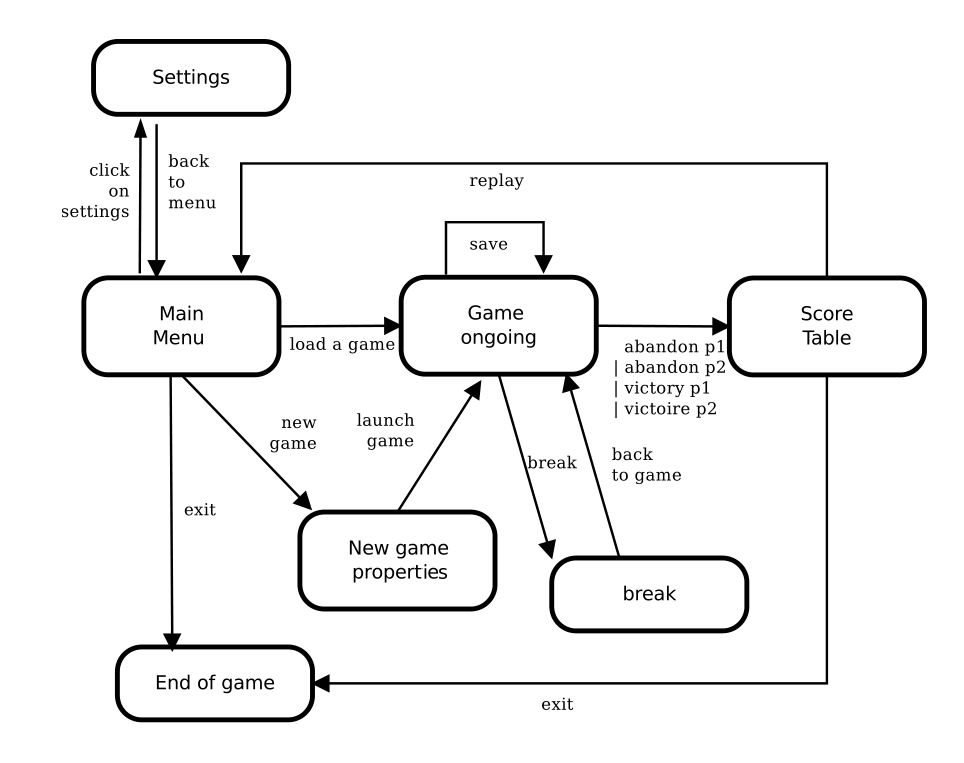
\includegraphics[width=0.7\textwidth]{figure/etat_transition.png}
			\end{center}
			\caption{Diagrame d'états-transitions du jeu.}
			\label{fig:transition_jeu}
		\end{figure}
	
		


		\subsection{Lancement du jeu}

		Au lancement de \emph{Bedbihan}, l'utilisateur peut débuter une nouvelle partie ou reprendre une partie préalablement sauvegardée. Le lancement d'une nouvelle partie implique de choisir une taille de carte et de sélectionner un peuple pour chacun des joueurs. Ceci est illustré par le diagramme d'utilisation de la {\sc Figure} \ref{fig:use1}.

		\begin{figure}
			\begin{center}
				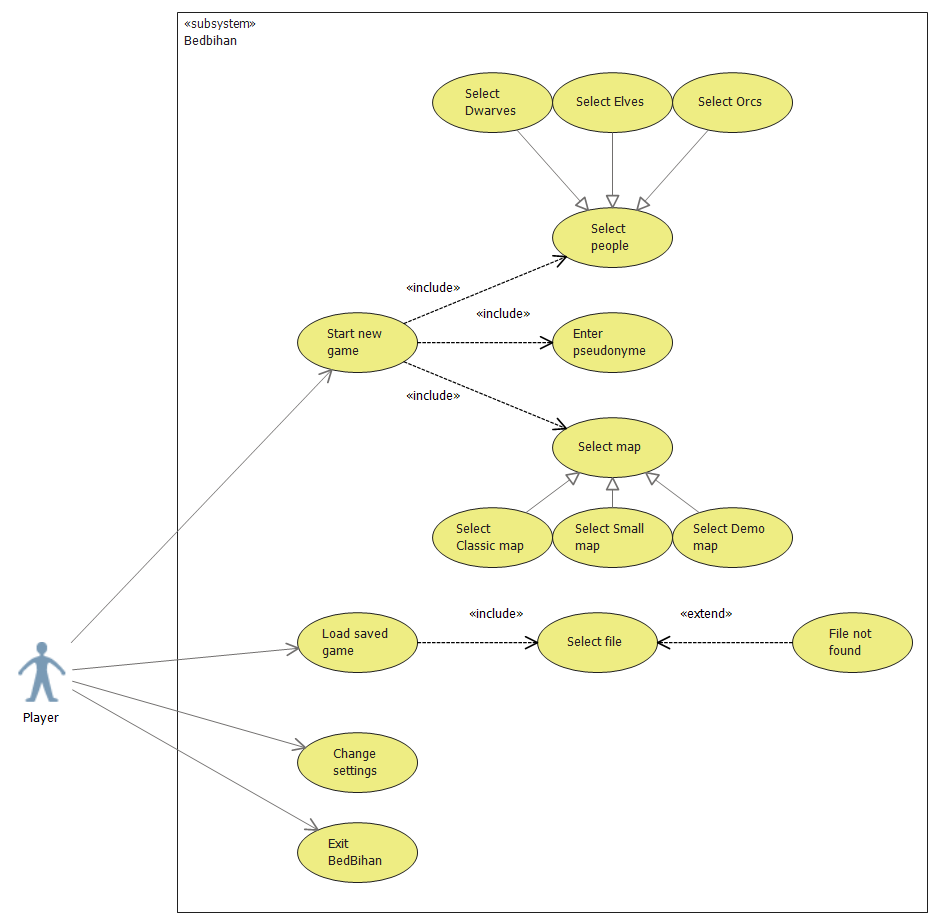
\includegraphics[width=1\textwidth]{figure/cas_utilisation_launch.png}
			\end{center}
			\caption{Actions possibles lors du démarrage du jeu.}
			\label{fig:use1}
		\end{figure}


	\subsection{Déroulement d'un tour pour un joueur}

		\emph{BedBihan} se jouant à tour de rôle, chaque joueur dispose de différentes actions possible lorsque c'est à lui de joueur. Les différentes possibilités sont illustrées par le diagramme d'utilisation présenté en {\sc Figure} \ref{fig:use2}.

		\begin{figure}
			\begin{center}
				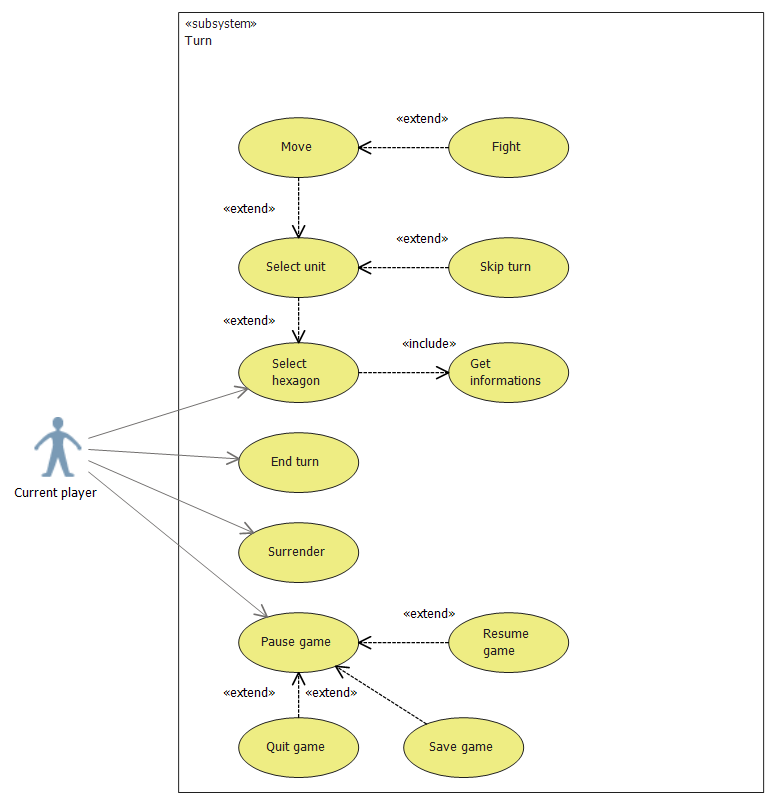
\includegraphics[width=1\textwidth]{figure/cas_utilisation_player_turn.png}
			\end{center}
			\caption{Actions possibles pour un joueur lors d'un tour.}
			\label{fig:use2}
		\end{figure}

	\subsection{Cycle de vie d'une unité}

	Les unités d'un joueur ont un cycle de vie illustré par le diagramme d'activité en {\sc Figure} \ref{fig:arbre_exemple_1}.


	\begin{figure}[h]
	            \centering
	            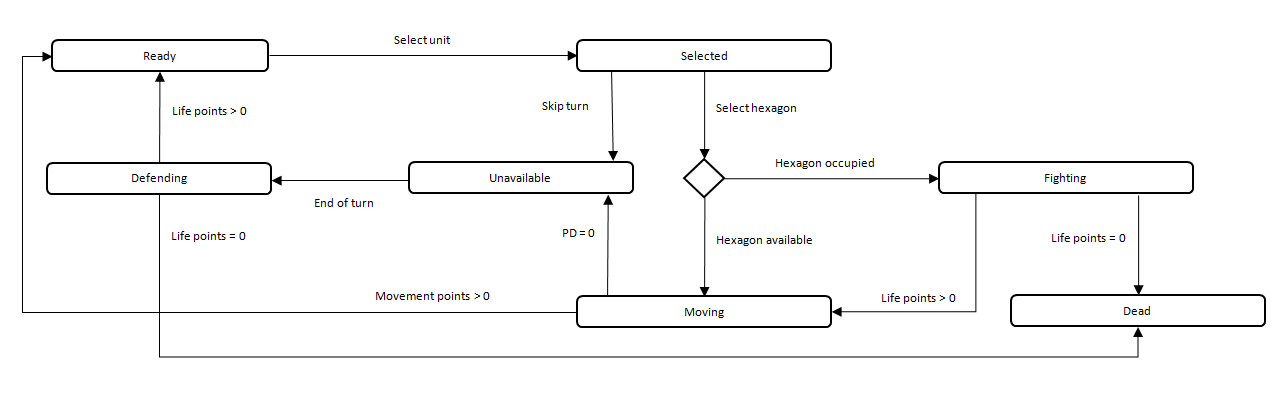
\includegraphics[width=1\textwidth]{figure/unit_life_cycle_state_diagram.png}
	            \caption{Cycle de vie d'une unité.}
	            \label{fig:arbre_exemple_1}
	\end{figure}